Usually we design our softwares thinking that they will run on a single \textit{executor}. However the increase of data sizes, and the consequent needs for architectures that can do efficient computations, determined the birth of a new programming model: \textbf{parallel computing}. The main idea at the basis of this model is that if a single computer is not able to compute operations on a huge quantity of data, so we can connect more and more computers in \textit{parallel} to get our computation done. Indeed, by now we have parallelism at several levels of our architectures. For example modern CPUs are designed with the aim of executing parallel code and also GPUs can be used for this purpose. However, in this work we are mainly focused on \textbf{clusters} of supercomputers, as we will see in detail in Section~\ref{sec22:parallelArchitectures}. In this chapter we will also study one of the most important tools for parallel computing: MPI

\section{Principles of parallel computing}\label{sec22:parallelComputing}

As we have seen in previous chapters, big data are deeply changing computer science and all its branches. So to deal with this new challenge we need to rethink our programming models and, how we have read in the introduction to this chapter, \textbf{parallel computing} can be an answer to these requests. According to \cite{Eijkhout}, parallel computing is simply an answer to the following problem: if there are $n$ operations to be done ans they would take time $t$ on a single processor, can they be done in time $t/p$ on $p$ processors?.\\

We use a parallel computer for two important reasons: to \textit{have access to more memory} and to \textit{obtain higher performance}. While it is simple to understand the gain in memory, as the total memory is the sum of the individual memories, the speed is harder to characterize. First of all we can give the following definition:

\begin{definition}[Speedup]
 Given $T_{1}$ as the best time to solve a problem in a single processor, and $T_{p}$ as the best solving time for the same problem with $p$ processors, we define the \textbf{speedup} $S_{p}$ as: $S_{p} = \frac{T_{1}}{T_{p}}$. 
\end{definition}

As we can see in the definition, we usually use different algorithms on different architectures in order to obtain the most efficient code possible. In the ideal case, $T_{p} = \frac{T_{1}}{p}$ (\textbf{perfect speedup}) but in practice is very difficult to obtain it, so $S_{p} \leq p$. To measure how far we are from the ideal speedup we can introduce the \textbf{efficiency} as $E_{p} = \frac{S_{p}}{p}$. As we can see $0 < E_{p} \leq 1$.\\

One of the reasons why we do not have perfect speedup, is that parts of a code can be inherently sequential. Supposing that 5\% of a code is sequential, then the time for that part cannot be reduced. Thus the speedup on that code is limited to a factor of 20. This phenomenon is described by the \textbf{Amdahl's Law}. According to \cite{Eijkhout} we can use the following definition:

\begin{definition}[Amdahl's law]
 Let $F_{s}$ be the sequential fraction and $F_{p}$ be the parallel fraction of a code. Then $F_{p} + F_{s} = 1$. The parallel execution time $T_{p}$ on $p$ processors is the sum of the part that is sequential ($T_{1}F_{s}$) and the part that can be parallelized ($T_{1}\frac{F_{p}}{p}$):
 \begin{equation}
  T_{p} = T_{1}(F_{s} + \frac{F_{p}}{p})
 \end{equation}
\end{definition}

When we have $p \rightarrow \infty$, the parallel execution time tends to $T_{1}F_{s}$, so the upper bound for the speedup is $S_{p} \leq \frac{1}{F_{s}}$.

\begin{figure}[htb] %  figure placement: here, top, bottom
   \centering
   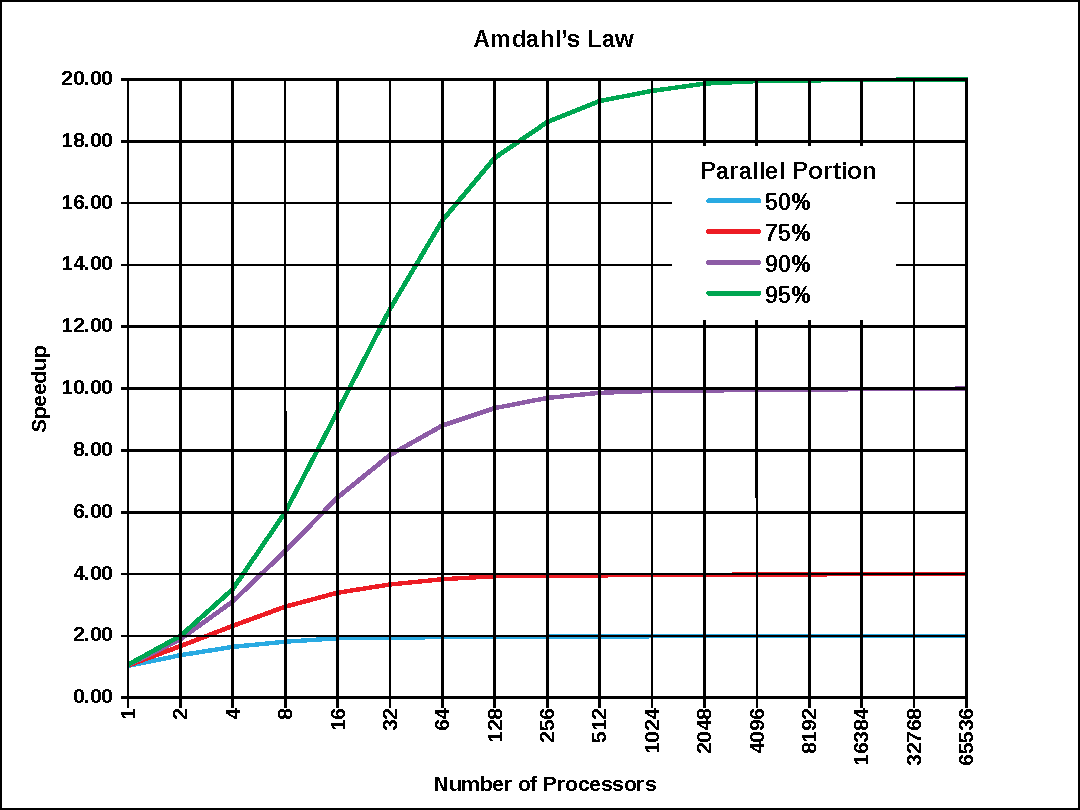
\includegraphics[width=0.70\linewidth]{images/AmdahlsLaw.pdf}\\
   \caption[Amdahl's Law]{Amdahl's Law. Image taken from Wikipedia}
   \label{fig:AmdahlsLaw}
\end{figure}

Amdahl's law is optimistic. In fact code parallelization give a speedup, but it also introduces communication overhead between processes. So if $T_{c}$ is the time spent on communication, we have:
\begin{equation}
 T_{p} = T_{1}(F_{s} + \frac{F_{p}}{p}) +  T_{c}
\end{equation}

Assuming we have a fully parallelized code, we can write:
\begin{equation}
 S_{p} = \frac{T_{1}}{T_{1}/p + T_{c}}
\end{equation}

Thus, to be close to $p$ we need $T_{c} \ll T_{1}/p$ or $p \ll T_{1}/T_{c}$.\\

As a consequence of the Amdahl's Law, our speedup is limited, so we do not have a great improvement with large-scale supercomputers. So now we are wondering why we should use parallel computing. In fact, when dealing with big data, we are not only interested in speedup but also in \textit{memory gain}. So, using this technique we are sure that our algorithms can finish returning a result. In this work, a primary importance is given to the improvement of memory occupation, as the three-dimensional models that we will create can be huge.

\section{Typical architectures for parallel computing}\label{sec22:parallelArchitectures}

Now we are interested in studying the most common architectures for parallel computing. A good source for this argument is \cite{Matloff}. How we can see there, these architectures are commonly divided into two groups: \textbf{shared-memory systems} and \textbf{message-passing systems}

\subsection{Shared-memory systems}

With this architecture, many CPUs share the same physical memory. So we talk about \textbf{MIMD}, which stands for \textit{Multiple Instruction Multiple Data}. In fact we have many different independent CPUs which access different memory locations at any given time. In these days, shared-memory systems are very common even on consumer PCs and mobile phones.\\

As an example we can consider a program which has a global variable $X$ and a local variable $Y$ on this hardware. If the compiler assigns location $200$ to $X$, then all processors will have that variable in common. In fact, any processor which issues a memory operation on location $200$ will access the \textit{same physical memory cell}. On the other hand, each processor will have its own run-time stack. All stacks are in shared memory, but they are accessed separately as each CPU has a different value in its stack pointer. Thus each processor will have its own independent copy of the local variable $Y$.\\

From a parallel point of view, each execution of a program requires parallel accessing of memory in order to avoid slowdowns. In parts this is handled by having a cache at each CPU, but it is also facilitated by dividing the memory into separate modules or \textit{banks}. The division can be done with two main strategies:
\begin{itemize}
 \item \textbf{High-order interleaving}: consecutive words are in the same bank (except at boundaries). It is widely used when dealing with matrices.
 \item \textbf{Low-order interleaving}: consecutive addresses are in consecutive banks (except when we get to the right end). It is widely used in GPUs
\end{itemize}

For a better understanding of shared-memory systems we can do the following example. Suppose we have to implement a matrix-vector multiplication between a vector $X$ and a matrix $A$ producing vector $Y$. The arrays for $A$, $X$ and $Y$ are held in common by all nodes. Then, each node multiply its assigned rows of $A$ times $X$ and place the result directly in the proper section of $Y$. From a technical point of view, these operations are usually done with \textit{threads}.

\subsection{Message-passing systems}

In message-passing systems, we have a certain number of independent CPUs each with its own independent memory. All processors communicate using some kind of network protocol. A typical environment for these systems is a \textbf{cluster} of different PCs. The idea consists in taking several PCs and networks and divide the computation sending \textbf{messages} to them containing their part of input data. Obviously, we need a fast network to avoid slowdowns due to network communication. The common choice today is \textit{Infiniband} as the traditional TCP/IP networks are quite slow. The common paradigm used in message-passing systems is the \textbf{scatter/gather paradigm}. According to this paradigm, we have a \textit{manager} node which sends out chunks of work to the other nodes, which are called \textit{workers}. When they have finished their work, workers send back to the manager the results which will be collected and assembled.\\

Now we can consider the same example as above of matrix-vector multiplication. With this architecture one node (for example node $0$) distributes the rows of $A$ to the other ones, so that each node receive a different set of rows, and the vector $X$ to all nodes. Each node then multiply $X$ by its own assigned rows of $A$ and then send back the results to node $0$ which will collect all parts and store in $Y$ the final result\\

As this type of architecture is the one chosen for our software, we will describe it more deeply when we will see the most important technology for implementation of a message-passing system: MPI.

\section{The Message Passing Interface}\label{sec22:MPI}

According to \cite{Matloff}, the \textbf{message-passing interface} or \textbf{MPI}, is a set of API called from user programs which provides a communication protocol for message-passing systems. So it is able to abstract all communications between processes. In MPI abstraction, when we write a program which will be run on four machines of the clusters, every machine  executes its own copy of the program and following official terminology we say we have four \textbf{processes}. Though the nodes are all running the same program, they will likely be working on different parts of its data. This is called the \textbf{Single Program Multiple Data} (\textbf{SPMD}).\\

From an architectural point of view, one of the most important parts of MPI is the \textbf{communicator}. It connects group of processes in the MPI session giving to each one an independent identifier which is called \textbf{rank}. By default the rank 0 process belongs to the MPI process that starts the program. Moreover the communicator arranges these processes in an ordered topology.\\

MPI also provides powerful methods for \textbf{point to point communications}. An example is \texttt{MPI\_Send} function, which allows one process to send a message to a second process. These type of communications are useful in irregular communication (for example a master-slave architecture where the master sends new data task to a slave whenever the prior task is completed).\\

Moreover MPI provides functions for \textbf{collective communications}:
\begin{itemize}
 \item \texttt{MPI\_Bcast}: The root sends messages from a buffer to all other processes
 \item \texttt{MPI\_Scatter}: The root has a buffer message and splits it into $n$ parts (where $n$ is the number of processes), then send each part to the corresponding process.
 \item \texttt{MPI\_Gather}: It is the opposite of scatter, in fact the root fills a buffer concatenating $n$ messages
 \item \texttt{MPI\_Reduce}: As in the gather function the root fills the buffer with $n$ messages. However, the collected data is then "reduced" using an associative function and the function returns the resulting value-
\end{itemize}


